% Página de copyright

{\small
\setlength{\parindent}{0em}\setlength{\parskip}{1em}
~
\vfill

% Data da primeira publicação
Primera edición, \editionyear{}

% Copyright
Copyright \copyright{} 2024 \authorname

% Texto resumido da licença
El folklore argentino es una rica expresión de nuestra historia y tradiciones. Con este proyecto, nos proponemos rescatar y poner en valor las canciones que han marcado a varias generaciones, contribuyendo así a mantener viva nuestra cultura popular y a fomentar el aprecio por nuestras raíces. Este proyecto es una construcción colectiva. Si tienes alguna sugerencia o corrección, por favor, comparte tus conocimientos escribiéndome a sestofrancisco@gmail.com.

% ISBN, se houver
\ifx\isbn\undefined\else\if\relax\detokenize\expandafter{\isbn}\relax\else{ISBN \isbn{}}\fi\fi

% Logotipo da editora
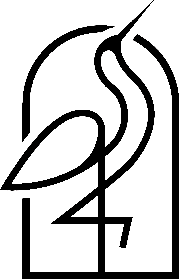
\includegraphics[width=0.07\linewidth]{frontmatter/logo-black.png}

% Editora
Publicado por \publisher{}
}
